% Chapter 3.2: External Aerodynamics and Surface Flows
% Part III of the book.

\chapter{External Aerodynamics and Surface Flows}
\label{ch:part3-external-aerodynamics-and-surface-flows}
\label{sec:aerodynamics}
% -----------------------------------------------------------------------------

Of the multi-query workflows \chapref{ch:part3-the-multi-query-bottleneck-in-computationa}
prices, the aerodynamic design sweep is the least forgiving, because most of its cost is work
that cannot be shared between queries. A shape change invalidates the mesh, the mesh invalidates
the solve, and the solve is a nonlinear iteration whose starting point does not transfer
cleanly from the previous shape. \index{aerodynamic shape optimization}
\index{external aerodynamics} What the sweep must produce, moreover, is small: an integrated
force coefficient, one number per geometry, obtained by integrating a field that had first to
be computed over every square centimeter of an irregular surface and millions of control
volumes around it. The classical machinery that produces those scalars is computational fluid
dynamics (CFD), and this chapter treats it as a competing implementation rather than as a straw
man. \index{computational fluid dynamics (CFD)}
That asymmetry --- an enormous machinery of approximation in service of a
handful of scalars --- is what makes this the natural first application for the surrogate
construction of Parts~I and~II, and it is also what makes the honest accounting awkward.
This chapter supplies both halves of the accounting.

The reader should bring the incompressible Navier--Stokes equations read as a solution
operator in \chapref{ch:part1-partial-differential-equations-as-solution}, the stationarity
requirement
behind the spectral layer of \chapref{ch:part1-the-fourier-neural-operator-spectral-theor}, the
discretization-invariance ledger of \chapref{ch:part1-discretization-invariance-and-continuum-li},
and the two graph interfaces built in \chapref{ch:part2-graph-neural-operators-gno-and-irregular-g},
whose point-to-grid and grid-to-point layers \eqref{eq:ch24-p2g}, \eqref{eq:ch24-g2p} are the
objects this chapter puts to work. Nothing here is proved; what is added to Part~II is the
physics the surrogate has to reproduce, the numbers attached to it with their sources pinned
down, and the axis along which a learned operator and a volume solver are actually comparable.
The route is short. Section~\ref{sec:ch32-formulation} fixes the governing system, the closure
that makes it solvable, and the two boundary conditions a body-fitted mesh must honor.
Section~\ref{sec:ch32-gino} states what the geometry-informed operator returns and what the
published aerodynamic evidence for it amounts to. Section~\ref{sec:ch32-comparison} sets the
surrogate and the finite volume pipeline side by side on four axes --- labor, wall-clock,
accuracy envelope, and certification ---; Section~\ref{sec:ch32-ledger} prices the amortization
those axes imply and records where the comparison breaks down.

% -----------------------------------------------------------------------------
\section{Physical Formulation and Boundary Conditions}
\label{sec:ch32-formulation}
% -----------------------------------------------------------------------------

Take a rigid body $\mathcal{B} \subset \mathbb{R}^3$ with surface $\partial\mathcal{B}$ moving
at constant speed through an otherwise quiescent Newtonian fluid, and write the flow in the
frame attached to the body, so that the far field is a uniform stream. For the road vehicles that
dominate this literature the freestream is tens of meters per second --- the simulation set of
Section~\ref{sec:ch32-gino} spans $10$ to $70\ \mathrm{m\,s^{-1}}$ --- which puts the Mach number
$U_\infty/a$ between $0.03$ and $0.2$ with $a \approx 340\ \mathrm{m\,s^{-1}}$; density variations
enter at order $(U_\infty/a)^2$, a few percent at worst, and are dropped, so the flow is treated as
incompressible. That is a modeling decision with a hard boundary: transonic aircraft cruise,
compressors, and any problem with shock waves fall outside it, and a surrogate trained on
incompressible, Reynolds-averaged labels has no obligation to warn when it is asked about them.
\index{incompressible flow!validity at low Mach number}
The steady Reynolds-averaged Navier--Stokes (RANS) equations for the mean velocity
$\mathbf{u}$ and mean pressure $p$ in the fluid region $\Omega \setminus \mathcal{B}$, with
$\Omega$ a bounded outer domain containing $\mathcal{B}$, are then
\index{Reynolds-averaged Navier--Stokes (RANS) equations}
\begin{equation}
  \label{eq:rans}
  \begin{cases}
    \rho (\mathbf{u} \cdot \nabla) \mathbf{u} = -\nabla p + \nabla \cdot \big( (\mu + \mu_t) (\nabla \mathbf{u} + \nabla \mathbf{u}^T) \big), & x \in \Omega \setminus \mathcal{B}, \\
    \nabla \cdot \mathbf{u} = 0, & x \in \Omega \setminus \mathcal{B},
  \end{cases}
\end{equation}
with $\rho$ the density, $\mu$ the molecular viscosity, and $\mu_t$ an eddy viscosity carrying
the effect of the unresolved turbulent fluctuations. Equation \eqref{eq:rans} is not a closed
system, and the reason is structural rather than cosmetic: averaging the Navier--Stokes
equations produces the Reynolds stress $\overline{\mathbf{u}' \otimes \mathbf{u}'}$ of the
fluctuation field, which is an unknown of the same order of magnitude as the mean stress in the
wake of a bluff body. The standard closure --- the Boussinesq hypothesis --- postulates a
scalar eddy viscosity,
\begin{equation}
  \label{eq:ch32-reynolds-stress}
  -\rho\, \overline{u_i' u_j'} = \mu_t \left( \frac{\partial u_i}{\partial x_j} + \frac{\partial u_j}{\partial x_i} \right) - \tfrac{2}{3} \rho k\, \delta_{ij},
  \qquad \mu_t = \frac{\rho k}{\omega} \ \text{(blended)},
\end{equation}
where $k = \tfrac{1}{2}\overline{u_i' u_i'}$ is the turbulent kinetic energy, $\omega$ the
specific dissipation rate, $\delta_{ij}$ the Kronecker symbol, and the parenthetical records
that the shear-stress transport (SST) variant blends two closures across the boundary layer.
\index{eddy viscosity}\index{Boussinesq hypothesis}\index{k--omega turbulence model}
Equation \eqref{eq:ch32-reynolds-stress} is completed by two further transport equations for
$k$ and $\omega$, solved simultaneously with \eqref{eq:rans}; they are not written here because
nothing in the surrogate depends on their form. What does depend on the closure is the accuracy
ceiling, and that point returns in Section~\ref{sec:ch32-ledger}.

The dimensionless group that sets the difficulty of \eqref{eq:rans} is the Reynolds number
\begin{equation}
  \label{eq:ch32-reynolds}
  Re = \frac{\rho U_\infty L}{\mu} \sim 10^5 - 10^7,
\end{equation}
the ratio of inertial to viscous force scales, with $L$ a body length\index{Reynolds number}.
The numerical content of \eqref{eq:ch32-reynolds} is
in the boundary layer. Viscosity is confined to a wall-attached layer of thickness
$\delta \sim L\,Re^{-1/2}$, so at $Re = 10^7$ and $L = 4.7\ \mathrm{m}$ --- a full-scale sedan
--- the layer is of order $1.5\ \mathrm{mm}$, three and a half orders below the body. A discretization that
is uniform in $L$ resolves nothing inside it. The wall-normal resolution a solver must therefore
achieve is conventionally stated in viscous units,
\begin{equation}
  \label{eq:ch32-yplus}
  y^{+} = \frac{\rho\, u_\tau\, y}{\mu},
  \qquad u_\tau = \sqrt{\tau_w / \rho},
\end{equation}
where $y$ is the distance from the wall, $\tau_w = \|\boldsymbol{\tau}_w\|$ the wall shear
stress (WSS) magnitude defined below, and $u_\tau$ the friction velocity. Closures integrated to the
wall, including the SST model used to generate the data of Section~\ref{sec:ch32-gino}, ask for
$y^{+} \lesssim 1$ at the first cell center. Inserting representative numbers ---
$\nu = \mu/\rho \approx 1.5\times 10^{-5}\ \mathrm{m^2\,s^{-1}}$,
$U_\infty \approx 40\ \mathrm{m\,s^{-1}}$, and a skin-friction coefficient of order
$3\times 10^{-3}$, so that
$u_\tau \approx 1.5\ \mathrm{m\,s^{-1}}$ --- puts the required first-cell height near
$10^{-5}\ \mathrm{m}$. Those are estimates, not measurements, but the span between them and the
body length $L$ is the whole reason a mesh, rather than a solver, is the rate-limiting stage of
an aerodynamic sweep. \index{boundary layer!thickness scaling}\index{mesh refinement!near-wall, viscous units}

Two conditions close the problem. On the body, (i) the no-slip wall condition
$\mathbf{u}(x) = 0$ for all $x \in \partial\mathcal{B}$\index{no-slip condition}; at the inflow,
(ii) the free-stream condition
\index{free-stream condition}
$\mathbf{u}(x) \to U_\infty \hat{\mathbf{e}}_x$ and $p(x) \to p_\infty$ as
$\|x\| \to \infty$. In practice (ii) is imposed on a finite outer boundary several body lengths
away, and the truncation is itself a numerical choice whose effect on the reported coefficients
is checked by enlarging the domain --- a mesh- and domain-convergence study of exactly the kind
Section~\ref{sec:ch32-ledger} finds no counterpart for on the surrogate side. Condition (i)
is where the two pipelines differ most sharply in mechanism: a finite volume code imposes it on
the faces of cells that conform to $\partial\mathcal{B}$, whereas an operator learns it as a
statistical property of the labels.

The engineering targets are not fields but three numbers. With $A_{\text{ref}}$ a reference
area --- usually the frontal projection for a road vehicle --- and $\tfrac{1}{2}\rho U_\infty^2$
the dynamic pressure,
\begin{equation}
  \label{eq:ch32-force-coeff}
  C_d = \frac{2 F_d}{\rho U_\infty^2 A_{\text{ref}}}, \qquad C_l = \frac{2 F_l}{\rho U_\infty^2 A_{\text{ref}}}, \qquad F_d = \int_{\partial\mathcal{B}} \big( -p \hat{\mathbf{n}} + \boldsymbol{\tau}_w \big) \cdot \hat{\mathbf{e}}_x \, dA,
\end{equation}
where $C_d$ and $C_l$ are the drag and lift coefficients, $F_d$ and $F_l$ the corresponding
forces, $\hat{\mathbf{e}}_x$ the unit vector along the freestream, $p$ the surface pressure,
$\boldsymbol{\tau}_w$ the wall shear stress, and $\hat{\mathbf{n}}$
the outward unit normal. The integrand of \eqref{eq:ch32-force-coeff} decomposes the drag
into a form or pressure part, governed by the pressure difference between the front face and the
recirculating wake, and a friction part carried by $\boldsymbol{\tau}_w$, the tangential traction
\begin{equation}
  \label{eq:ch32-wss}
  \boldsymbol{\tau}_w = \big[ \boldsymbol{\sigma}\,\hat{\mathbf{n}} \big]_{\text{tan}},
  \qquad \tau_{w,t} = \mu \left. \frac{\partial u_t}{\partial n} \right|_{\partial\mathcal{B}},
\end{equation}
with $\boldsymbol{\sigma}$ the viscous stress tensor, $u_t$ the tangential velocity component,
and $n$ the wall-normal direction. The second identity in \eqref{eq:ch32-wss} is the one that
matters here: the friction contribution to \eqref{eq:ch32-force-coeff} is a \emph{normal
derivative} of the velocity field at the wall, so it is the quantity most sensitive to the
near-wall resolution \eqref{eq:ch32-yplus} makes expensive. \index{wall shear stress (WSS)}
\index{drag coefficient}\index{pressure drag and skin-friction drag}
A surrogate that predicts $p$ well and $\boldsymbol{\tau}_w$ poorly can still reproduce a
bluff-body $C_d$, because the pressure term dominates it; that is a reason to report the two
fields separately rather than only the integral.

% -----------------------------------------------------------------------------
\section{The GINO Aerodynamic Surrogate}
\label{sec:ch32-gino}
% -----------------------------------------------------------------------------

The object the surrogate is asked to learn is the map from a geometry and an operating condition
to the two surface fields that feed \eqref{eq:ch32-force-coeff},
\begin{equation}
  \label{eq:ch32-surrogate-map}
  \mathcal{G}_\theta : \big( \mathrm{SDF}_{\mathcal{B}},\, \mathbf{x},\, U_\infty \big)
  \longmapsto \big( p|_{\partial\mathcal{B}},\, \boldsymbol{\tau}_w|_{\partial\mathcal{B}} \big),
\end{equation}
where $\mathrm{SDF}_{\mathcal{B}}$ is the signed distance function (SDF) of the body and
$\mathbf{x}$ collects the surface coordinates\index{signed distance function (SDF)!as geometry channel}.
Equation \eqref{eq:ch32-surrogate-map} is the
aerodynamic instance of the generic layer of \eqref{eq:no_layer}, and it inherits the hypotheses
of the approximation theorems proved for that layer: the set of admissible inputs must be compact
in whatever norm the geometry is measured in, and nothing in Part~I fixes what the right norm on a
triangulated surface is.

The obstacle to using the Fourier machinery directly is geometric. A spectral layer presumes a
lattice and a stationary kernel \cite{kovachki2023neural,li2021fourier}; the surface of a car is
an irregular triangulation with no translational symmetry, and the fluid domain is exterior and
unbounded, so the periodic torus of \chapref{ch:part1-the-fourier-neural-operator-spectral-theor}
is not merely inconvenient but false. Rasterizing the body into a Cartesian box and running a
three-dimensional Fourier neural operator (FNO) on the box does not fix this cheaply: the box
must be fine enough to
resolve a boundary layer measured by \eqref{eq:ch32-yplus}, which makes most of its cells
empty space, and the cost of the transform is then paid almost entirely on vacuum. The
\textbf{Geometry-Informed Neural Operator (GINO)}
\cite{li2023geometry}\index{Geometry-Informed Neural Operator (GINO)!aerodynamic surrogate}
resolves this by mapping
the unstructured point cloud onto a regular 3D latent bounding grid via a continuous graph
operator, executing fast 3D spectral convolutions, and decoding back to surface vertices --- the
encoder \eqref{eq:ch24-p2g}, the latent Fourier stack, and the decoder \eqref{eq:ch24-g2p} of
\chapref{ch:part2-graph-neural-operators-gno-and-irregular-g}, with the geometry entering as
channels rather than as connectivity. The design consequence of that arrangement is that the
mesh is touched twice, at the two interfaces, and the expensive global mixing in between runs at
a resolution chosen independently of the tessellation. Where a body-fitted solver must rebuild
its grid for every shape, \eqref{eq:ch24-g2p} only needs new evaluation coordinates.

\begin{case_study}
\label{case:ch32-ahmed}
The published evidence for \eqref{eq:ch32-surrogate-map} comes from two families of vehicle
geometries \cite{li2023geometry}. The first is a set of more than five hundred Ahmed-body
variants\index{Ahmed body} generated for the study by Latin-hypercube sampling over six design
parameters --- length, width, height, ground clearance, slant angle, and fillet radius --- together
with the inlet velocity; each surface carries $\mathcal{O}(10^{5})$
nodes and each
flow field $\mathcal{O}(10^{7})$ volume cells (7.2 million mesh points, of which 100{,}000 are on
the surface, in the configuration reported). The labels were produced with the GPU-accelerated
OpenFOAM solver run in steady mode with the SST $k$--$\omega$
closure of \eqref{eq:ch32-reynolds-stress}, at Reynolds numbers from $4.35\times10^{5}$ to
$6.82\times10^{6}$ --- the inlet velocities just mentioned, $10$ to $70\ \mathrm{m\,s^{-1}}$ --- at
a cost of 7--19 hours per geometry on 16 central processing unit (CPU) cores and two NVIDIA V100
GPUs. The second family is the
ShapeNet Car collection\index{ShapeNet Car dataset}, whose surfaces are stored with roughly
$3.7\times10^{3}$ nodes.
Trained on the Ahmed family, GINO reports a relative $L^2$ error of $8.31\%$ on the full surface
pressure field against $11.16\%$ for the best prior method; on the ShapeNet Car set it reports
$7.12\%$ against $9.42\%$ for a plain three-dimensional FNO, with the latent grid fixed at
$64^{3}$ for the grid-based models. The errors are in the metric of \eqref{eq:rel_l2_loss}.
\end{case_study}

Figure~\ref{fig:vol3_aero} shows the kind of object \eqref{eq:ch32-surrogate-map} returns.
Panel~(a) --- this chapter's subject --- renders a car body as its triangulated surface colored
by predicted static pressure, with external streamlines threading over the hood and roof and a
tangled bundle of them detaching behind the base. Panel~(b) is the atmosphere on the sphere, and
belongs to \chapref{ch:part3-global-weather-forecasting-and-climate-dyn}. The two are printed as
one figure because they mark the two ends of the design space this part occupies: the same
spectral machinery, needing a graph interface at each end on the lattice-free surface of
panel~(a) and none on the fixed sphere of panel~(b). The reading
panel~(a) should leave is qualitative but load-bearing. High pressure (red,
near the upper end of the $0$--$1000\ \mathrm{Pa}$ bar) sits at the front stagnation region on
the bumper and hood; the lowest pressures (violet, near the windshield base and the rear side
window) sit where the flow accelerates over curved surfaces, consistent with the pressure term
of \eqref{eq:ch32-force-coeff} being dominated by the front-to-base difference; and the
detached, coiled streamlines behind the car mark the wake, the region whose mean pressure sets
the drag and whose RANS prediction is least reliable. Two cautions belong with the figure. The
two color bars under panel~(a) are not mutually consistent --- a pressure span of order $10^{3}\ \mathrm{Pa}$ is
what a freestream near $40\ \mathrm{m\,s^{-1}}$ would generate through the dynamic pressure
$\tfrac{1}{2}\rho U_\infty^{2}$ in air at standard density, whereas the velocity bar saturates at
$2\ \mathrm{m\,s^{-1}}$ --- and panel~(a) is a rendering
of the output type, not a quantitative solver comparison. Nothing in the argument below rests
on it.

\begin{figure}[htbp]
\centering
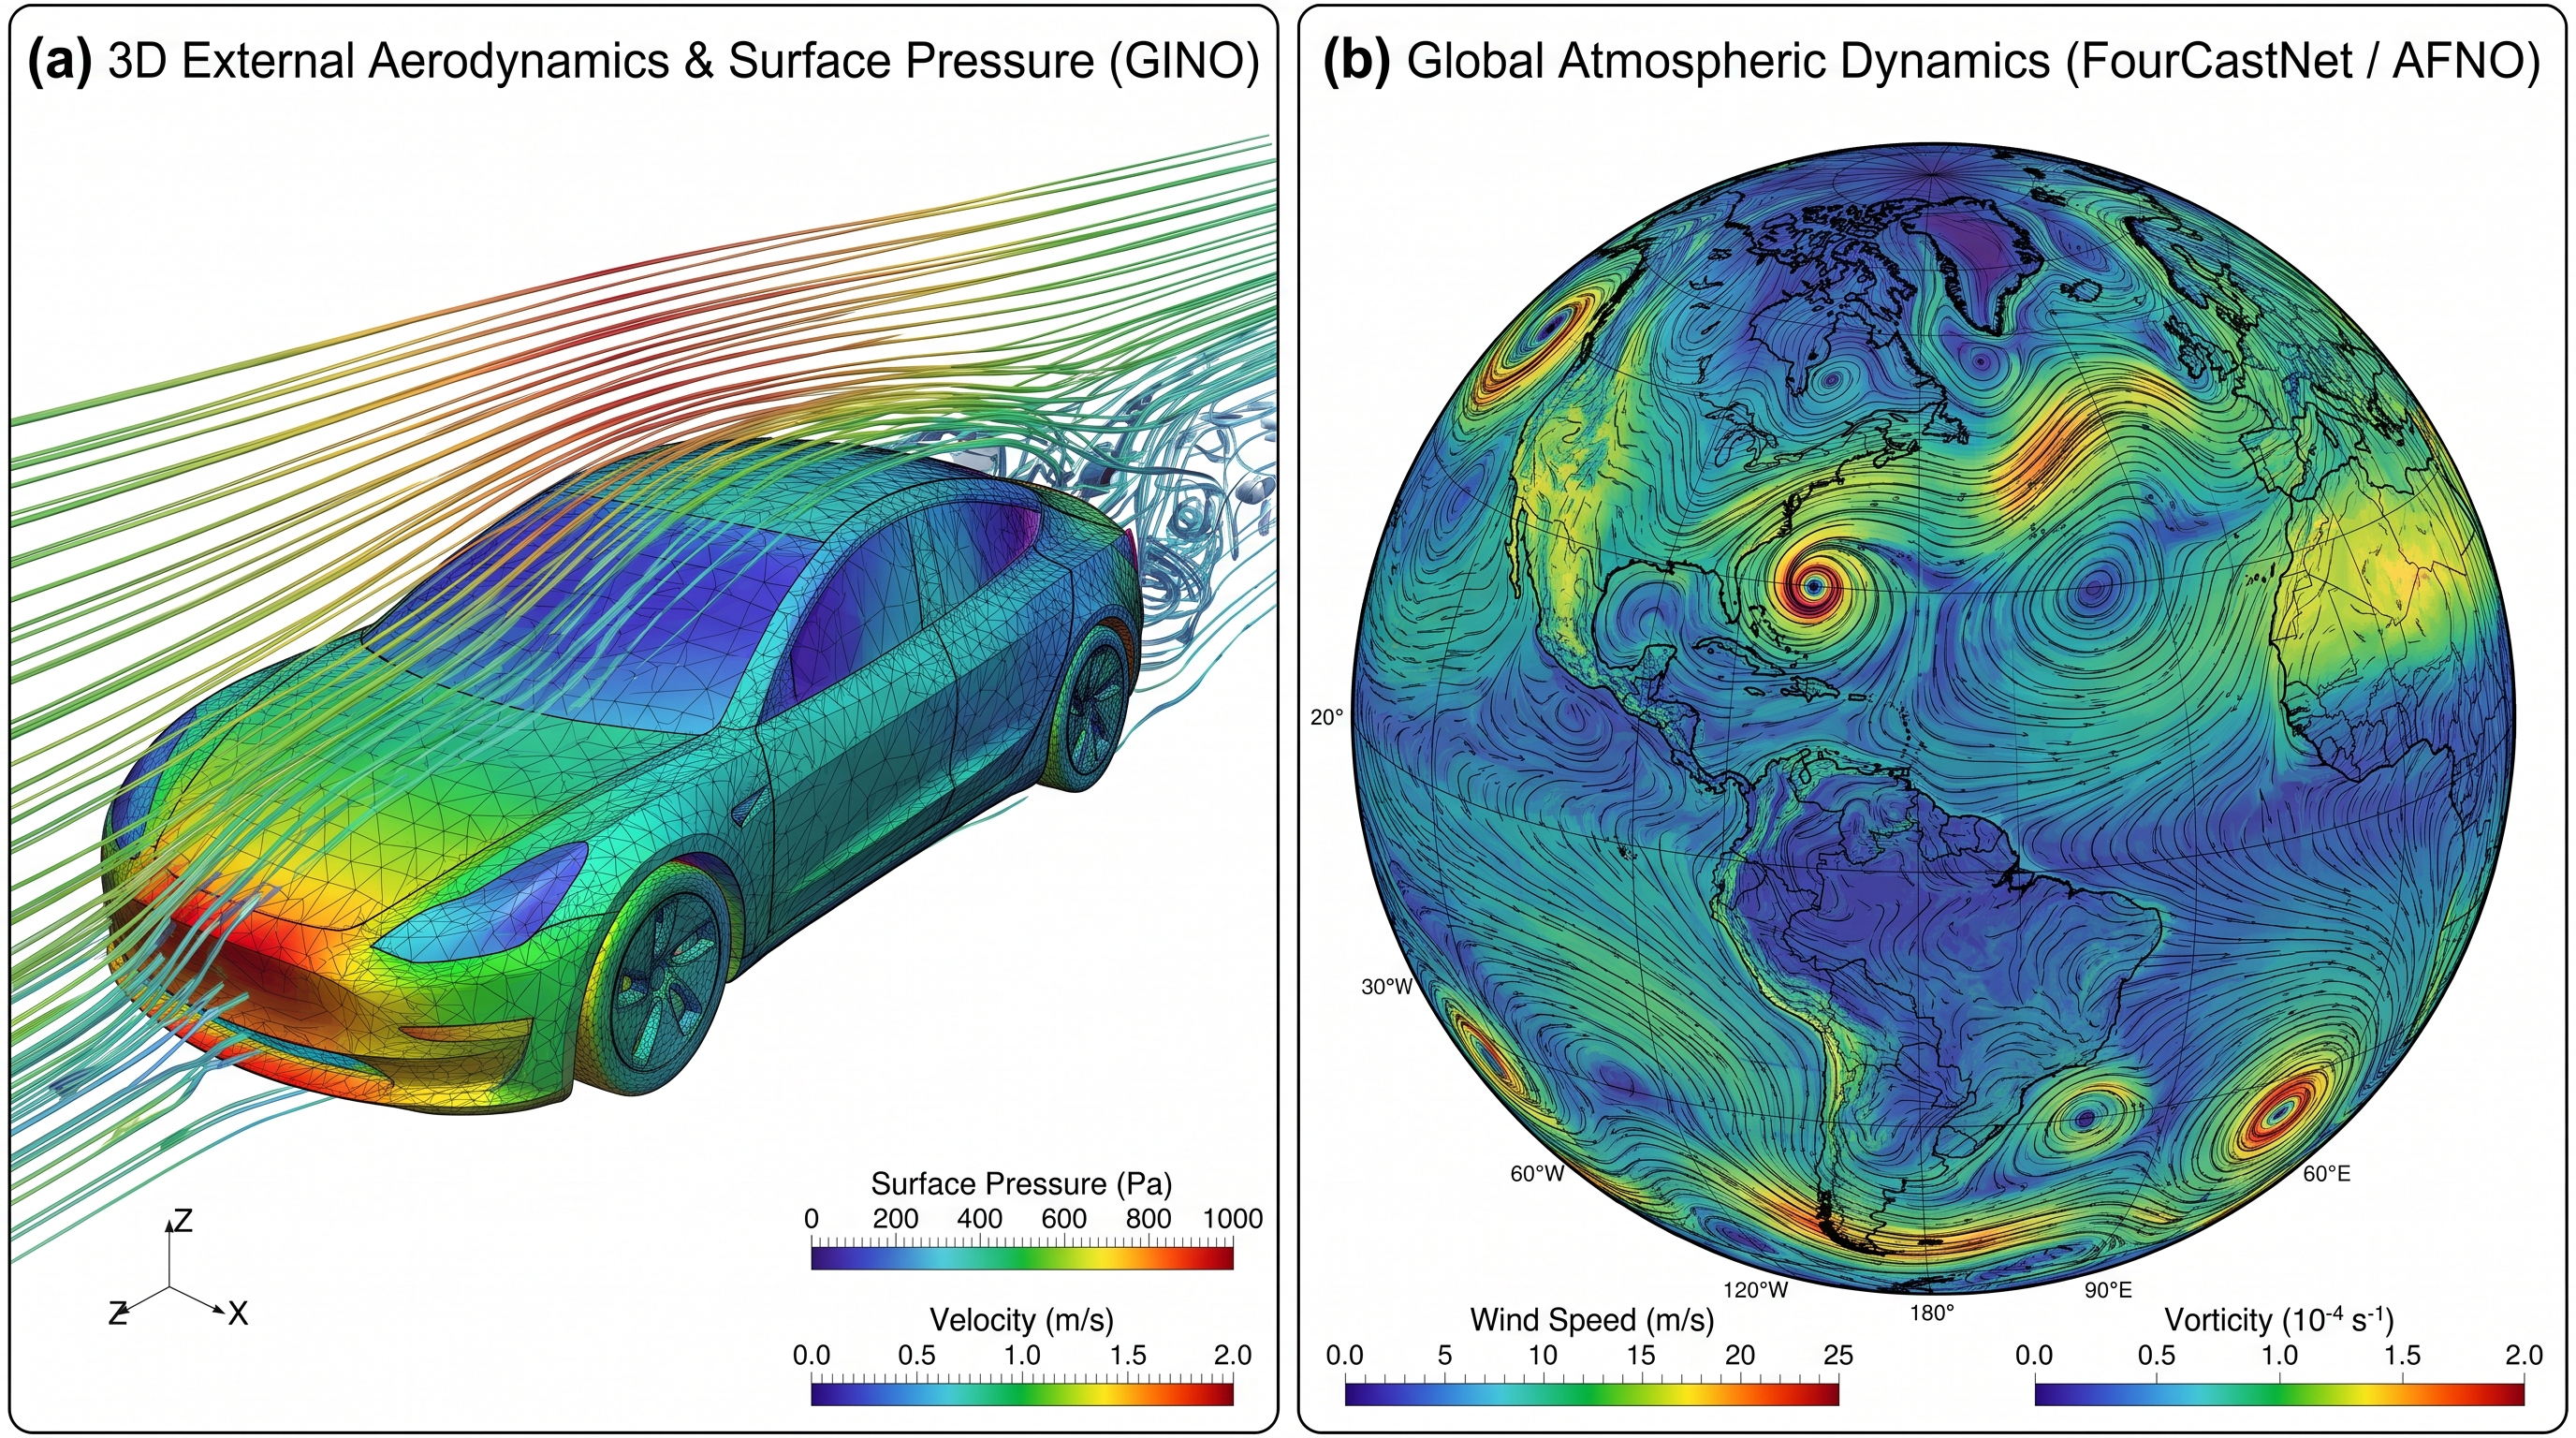
\includegraphics[width=0.95\textwidth]{fig_vol3_aerodynamics.jpg}
\caption{\textbf{Two-panel figure: surface pressure on a vehicle body (panel (a)) and global atmospheric structure (panel (b)).} Panel~(a), the subject of this chapter, renders the car body as its triangulated surface and colors it by predicted static pressure in pascals (color bar, $0$--$1000\ \mathrm{Pa}$); the external streamlines are colored by flow speed in meters per second (color bar, $0$--$2\ \mathrm{m\,s^{-1}}$), with the body axes at lower left. High pressure concentrates over the front bumper and hood, low pressure over the windshield and rear side window, and the flow detaches into a wake behind the base --- the front-to-base pressure difference that carries most of the drag on a bluff body. Panel~(b), the subject of \chapref{ch:part3-global-weather-forecasting-and-climate-dyn}, is a near-side view of the Earth with wind speed as shading and vorticity as contours, the fixed-sphere counterpart of the irregular geometry in panel~(a); it is cited from \chapref{ch:part3-global-weather-forecasting-and-climate-dyn} for that reading. Panel~(a) is an illustrative rendering of the output of a geometry-informed surface surrogate (GINO) of the type built in \chapref{ch:part2-graph-neural-operators-gno-and-irregular-g} and evaluated in Case Study~\ref{case:ch32-ahmed}; the two color bars beneath it are not mutually consistent and it is not a solver result.}
\label{fig:vol3_aero}
\end{figure}

Two further properties of the construction are aerodynamically useful and are worth stating
with their limits. The first is resolution behavior. GINO is discretization-convergent in the
sense of \cite{li2023geometry}: trained and tested at latent resolutions from $32$ to $88$, the
reported error is roughly flat, whereas a three-dimensional U-Net degrades at low resolution
because its receptive field shrinks with the grid; and trained on meshes sub-sampled by factors
of $2$ to $8$, the model evaluated on the full tessellation holds its error --- the zero-shot
super-resolution of \chapref{ch:part1-discretization-invariance-and-continuum-li} applied to a
surface rather than a volume. The caveat of that chapter transfers intact. Sub-sampling a mesh
thins the \emph{sampling} of a fixed smooth geometry; it does not remove geometric detail, and
the claim is therefore resolution transfer, not recovery of features absent from the coarse
input\index{zero-shot super-resolution!on surface meshes}.
The second is the alternative the
architecture did not take. Mesh-based message-passing solvers
\cite{brandstetter2022message} stay on the solver's own connectivity and never need a latent
box; GINO pays $\mathcal{O}(|E|)$ graph work --- $|E|$ the edge count of the two interface graphs
--- at two thin interfaces to buy a transform, and the
choice is exactly the one \chapref{ch:part2-graph-neural-operators-gno-and-irregular-g} prices.
For exterior aerodynamics the transform is worth it because the wake couples the base to the
far field, and a radius-$r$ graph layer needs many compositions to carry that interaction.

% -----------------------------------------------------------------------------
\section{Comparison with Classical Solvers (FVM / OpenFOAM)}
\label{sec:ch32-comparison}
% -----------------------------------------------------------------------------

The baseline is a finite volume method (FVM) code, and the framing should be precise about what
the method guarantees\index{finite volume method (FVM)!conservation identity}.
A finite volume discretization integrates the balance laws over each
control volume, so mass and momentum are conserved cell by cell as an algebraic identity of the
update, independently of whether the solution is accurate, with the boundary conditions entering
through face values and ghost cells rather than as constraints on a trial space
\cite{leveque2002finite}. Whether the resulting coupled algebraic system is solvable to accuracy is
a property of that system --- the stability analysis of the discrete problem, which for the
incompressible coupling is a mixed-formulation question \cite{quarteroni2008numerical} --- and not
something inherited automatically from the continuum problem. For \eqref{eq:rans} the
pressure--velocity coupling is handled
by a splitting algorithm --- the semi-implicit method for pressure linked equations (SIMPLE)
and its variants, or the pressure--implicit with splitting of operators (PISO) scheme for
transient problems --- and the steady state is reached by $1{,}500$ to $3{,}000$ such outer
iterations, each of which solves a linear system\index{SIMPLE and PISO pressure--velocity coupling}.
Two properties of that pipeline are what a design office buys, and neither is supplied for free
by a surrogate: the conservation identity, visible in residuals a certifier can inspect, and a
mesh-convergence study, the discipline's standard evidence that a reported $C_d$ is not an
artifact of the grid\index{mesh convergence study}.

The comparison is therefore not a single number but four axes: the labor that scales with
geometry, the wall-clock per query, the accuracy envelope and how it is measured, and
certifiability\index{surrogate!versus classical solver, axes of comparison}.
On labor, the solver pipeline is dominated by geometry intake --- computer-aided design (CAD)
cleanup, surface triangulation, boundary-layer prisms satisfying \eqref{eq:ch32-yplus}, volume
meshing, and quality checks on skewness and orthogonality --- and none of it amortizes, because
every candidate shape invalidates the mesh. The surrogate keeps the obligation in reduced form:
\eqref{eq:ch32-surrogate-map} still needs a tessellation and an $\mathrm{SDF}_{\mathcal{B}}$,
but a surface one rather than a volume one. On wall-clock, the attributed figure is
the 7--19 hours per geometry for label generation reported in Case
Study~\ref{case:ch32-ahmed}, against the
$2.6\times10^{4}$ ratio the cost--accuracy analysis of \cite{li2023geometry} reports for
computing drag coefficients relative to that same GPU OpenFOAM solver, measured as
the inference time needed to reach a $3\%$ relative error in $C_d$\index{cost--accuracy trade-off}.
Three qualifications make
that ratio usable. It is quoted against an optimized GPU solver run of the same case, not against
a conventional CPU solve, so the two wall-clock figures in circulation for this workload are not
interchangeable; the same work's
conclusion quotes a factor nearer $10^{5}$, and the book keeps the smaller, cost--accuracy-based
figure. It excludes meshing on both sides, though not the surrogate's own geometry intake: the
reported evaluation time includes computing the signed distance function, running the model, and
integrating the drag. And it is a ratio of times at matched accuracy, not a
statement that the surrogate is accurate --- the accuracy in question is the $3\%$ drag error at
which both curves are read. A tighter agreement with the volume solve, $1.2\%$, is also quoted for
this workload, but it is not a number \cite{li2023geometry} reports, and this chapter does not use
it.

% -----------------------------------------------------------------------------
\section{Amortization, the Pipeline Ledger, and Four Failure Modes}
\label{sec:ch32-ledger}
% -----------------------------------------------------------------------------

One arithmetic check belongs here, because this workload circulates with more than one wall-clock
pairing. A second, common in the applications literature, is a body-fitted mesh of order
$2\times10^{7}$ cells, a solve of $15$--$45$ minutes on 64 CPU cores, and a surrogate
evaluation of order ten milliseconds on an NVIDIA A100. That pairing is not the one behind the
number above, and it does not reconstruct it --- $9\times10^{2}\ \mathrm{s}$ over
$1\times10^{-2}\ \mathrm{s}$ is $9\times10^{4}$, not $2.6\times10^{4}$. Nor does it match the
device and cost the cited work states, which are a single NVIDIA V100 and $0.1\ \mathrm{s}$ per
shape, an order of magnitude above the ten milliseconds just quoted. The two figures differ because
their baselines, their hardware, and their accuracy targets all differ.
The rule the chapter follows throughout is that a
speedup travels with the baseline and the accuracy target that produced it, or not at
all\index{speedup ratios!baseline and accuracy target}.

What ties the first two axes together is amortization, where the arithmetic of
\chapref{ch:part2-production-deployment-and-high-throughput-} applies unchanged. If
$C_{\text{train}}$ is the offline cost of fitting
\eqref{eq:ch32-surrogate-map} --- several hundred solver runs at 7--19 hours each, the dominant
term by far --- and $C_{\text{eval}} \ll C_{\text{solve}}$ are the per-query costs, the
break-even query count is
\begin{equation}
  \label{eq:ch32-break-even}
  N_q^{*} = \frac{C_{\text{train}}}{C_{\text{solve}} - C_{\text{eval}}},
  \qquad
  \frac{C_{\text{train}}}{N_q} + C_{\text{eval}} \;\le\; C_{\text{solve}} \iff N_q \;\ge\; N_q^{*}.
\end{equation}
Equation \eqref{eq:ch32-break-even} is the honest form of the speedup claim: the
$2.6\times10^{4}$ factor is $C_{\text{solve}}/C_{\text{eval}}$, not the amortized ratio, and a
benchmark on a handful of held-out shapes never reaches $N_q^{*}$; a shape optimization loop over
thousands of variants
does, which is the workflow \chapref{ch:part3-the-multi-query-bottleneck-in-computationa}
enumerated\index{break-even query count}.
Table~\ref{tab:ch32-pipelines} sets the pipelines side by side, and two rows carry the remaining
axes. The error-reference row records that a solver's accuracy envelope is established by grid,
domain, and time-step refinement whereas the surrogate's is a comparison against a fixed set of
labels, so by the budget \eqref{eq:ch27-budget} the surrogate cannot be better than the fields it
was trained on; the certification row records what a reviewer may ask of each.

\begin{table}[htbp]
\centering
\small
\caption{\textbf{Two routes to a drag coefficient for one geometry.} Times and counts are those reported in \cite{li2023geometry} for the Ahmed-body configuration of Case Study~\ref{case:ch32-ahmed}; the $15$--$45$ minute CPU pairing discussed in the text is not from that source.}
\label{tab:ch32-pipelines}
\begin{tabularx}{\textwidth}{@{}>{\raggedright\arraybackslash}p{0.20\textwidth}>{\raggedright\arraybackslash}X>{\raggedright\arraybackslash}X@{}}
\toprule
\textbf{Stage} & \textbf{RANS volume solver (FVM)} & \textbf{GINO surface surrogate} \\
\midrule
Geometry intake & CAD cleanup, surface wrap, prismatic boundary-layer cells at $y^{+} \lesssim 1$ & surface tessellation plus $\mathrm{SDF}_{\mathcal{B}}$; no volume mesh \\
Unknowns & $\mathcal{O}(10^{7})$ cells, $\mathcal{O}(10^{5})$ surface nodes & $\mathcal{O}(10^{5})$ surface nodes at the interfaces; $64^{3}$ latent grid inside \\
Physics & \eqref{eq:rans} with closure \eqref{eq:ch32-reynolds-stress}, solved simultaneously & closure never solved; its effect is absorbed into the labels \\
Solve & SIMPLE-type outer iterations, linear solves per step, residual monitoring & one forward pass; cost per field as \eqref{eq:ch27-cost} \\
Output & volume field $(\mathbf{u},p,k,\omega)$ everywhere, plus surface integrals \eqref{eq:ch32-force-coeff} & surface fields $(p,\boldsymbol{\tau}_w)$ only; $C_d$ obtained by quadrature \\
Wall-clock per geometry & 7--19 h on 16 cores and 2 GPUs (label generation) & $0.1\ \mathrm{s}$ per shape on one NVIDIA V100; $2.6\times10^{4}\times$ faster at $3\%$ drag error \\
Error reference & grid, domain, and time-step convergence & relative $L^2$ on surface pressure, $7$--$8\%$ on the two families \\
Certification hook & conservation identity, inspectable residuals, mesh study & no conservation guarantee; requires the (model, mesh, metric) triple of \chapref{ch:part2-graph-neural-operators-gno-and-irregular-g} \\
\bottomrule
\end{tabularx}
\end{table}

What remains are the failure modes, and they are specific to this application. The first is
distributional. The Ahmed body is a simplified bluff body: its underbody
is flat, its wheels are usually idealized, and its mirrors, door gaps, and cooling flows are
absent. A surrogate trained on that family and asked about a production car with a detailed
underbody returns a plausible field, not an error message --- the out-of-distribution (OOD)
failure\index{out-of-distribution (OOD) failure!geometry families}
\chapref{ch:part2-production-deployment-and-high-throughput-} warns about, here with a geometry
rather than a coefficient field as the argument. The second is the closure. Where RANS with
\eqref{eq:ch32-reynolds-stress} mispredicts separation --- and the base pressure of a bluff body
is precisely where a scalar eddy viscosity is most suspect --- the labels carry the error and
\eqref{eq:ch27-budget} makes it irreducible by retraining on the same
grid\index{turbulence model error!label ceiling}. A surrogate can be
made cheap; it cannot be made more faithful to the physics than the model that generated its
data, and the honest comparison is therefore against wind-tunnel measurement, which is what
industry does and which no operator-learning result in this book addresses. The third is
conservation: \eqref{eq:ch32-surrogate-map} never forms a flux balance, so the cell-by-cell
identity that \cite{leveque2002finite} makes structural in the finite volume update has no
counterpart here, and the predicted
pressure and WSS fields need not integrate consistently with any divergence-free velocity ---
the gap \chapref{ch:part3-boundary-condition-enforcement-neural-oper} takes up. The fourth is
scope: anything downstream that needs the volume --- acoustics, thermal loading, a force on a
component inside the engine bay --- is outside \eqref{eq:ch32-surrogate-map} however well the
surface is predicted.

\takeaway{What the Aerodynamic Numbers License}{The reported result is a surface surrogate that
reaches a $3\%$ drag error in wall-clock shorter by a factor of $2.6\times10^{4}$ than an
optimized GPU RANS run, at $7$--$8\%$ relative $L^2$ error on the surface pressure field, for a
family of bluff bodies at $Re \le 6.82\times10^{6}$. It is not a certified replacement for a
convergence study, it does not extend across geometry families without new labels, and its
accuracy is bounded by the turbulence model that produced those labels.}

% -----------------------------------------------------------------------------
% Bridge to Chapter 3.3
% -----------------------------------------------------------------------------

Every limitation just listed has a counterpart in a different domain, and the next chapter
makes the contrast productive. External aerodynamics as treated here is a boundary-value
problem: the designer wants the solution \emph{at} the boundary, on a geometry that varies from
query to query, with no initial condition at all because the steady state is what is reported;
the surrogate's job is a shape-to-surface-field map evaluated once per shape. Global atmospheric
prediction inverts both parameters. The geometry is
fixed --- the sphere $\mathbb{S}^2$, the one case where the lattice and stationarity assumptions
that \chapref{ch:part1-the-fourier-neural-operator-spectral-theor} surrendered for a car body are
available again, although \chapref{ch:part3-global-weather-forecasting-and-climate-dyn} is careful
to note that the availability is not free, because an equiangular latitude--longitude grid is not
the sphere --- and the state evolves, so the operator is a time-stepper applied forty times in
succession for a ten-day forecast and the error question becomes the rollout question of
\chapref{ch:part1-open-theoretical-problems-and-mathematical}. There the multi-query budget is
not thousands of geometries but fifty perturbed initial states twice a day, the labels are not
solver runs but a reanalysis --- a data-assimilation system cycled through the observational
record --- and the acceptance metric is not a drag coefficient but a skill score evaluated at a
lead time. The label-ceiling objection raised above returns there in a harsher register: a
reanalysis is the output of a primitive-equation core plus a tuned parameterization package plus
an assimilation system, so a surrogate trained on it inherits three error sources at once and,
unlike a finite volume solve, cannot be audited term by term. The conservation half of the
objection is deferred to \chapref{ch:part3-boundary-condition-enforcement-neural-oper}, which
treats it as a property a learned map may be built to satisfy rather than one it inherits.

% -----------------------------------------------------------------------------
